% ============================================================
%  FRAME TREE — TF hierarchy with hardware-based coloring
%  Requires: tikz
% ============================================================
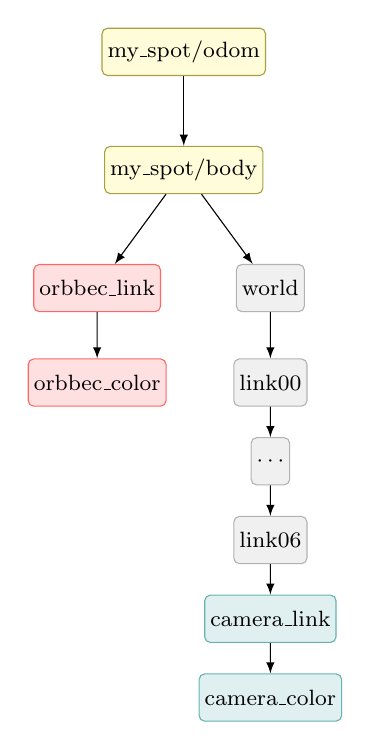
\begin{tikzpicture}[
    level 1/.style={sibling distance=40mm},
    level 2/.style={sibling distance=22mm},
    level 3/.style={level distance=12mm},
    level 4/.style={level distance=10mm},
    every node/.style={draw, rounded corners=2pt, font=\footnotesize,
                       inner sep=2pt, minimum height=6mm},
    edge from parent/.style={draw, -latex},
    spot/.style  = {fill=yellow!15,  draw=yellow!60!black},
    z1/.style    = {fill=gray!12,   draw=gray!60},
    orbbec/.style = {fill=red!12,   draw=red!60},
    rs/.style    = {fill=teal!12,   draw=teal!60},
  ]
  \node[spot] {my\_spot/odom}
    child { node[spot] {my\_spot/body}
      child { node[orbbec] {orbbec\_link}
        child { node[orbbec] {orbbec\_color} }
      }
      child { node[z1] {world}
        child { node[z1] {link00}
          child { node[z1] {$\cdots$}
            child { node[z1] {link06}
              child { node[rs] {camera\_link}
                child { node[rs] {camera\_color} }
              }
            }
          }
        }
      }
    };
\end{tikzpicture}
